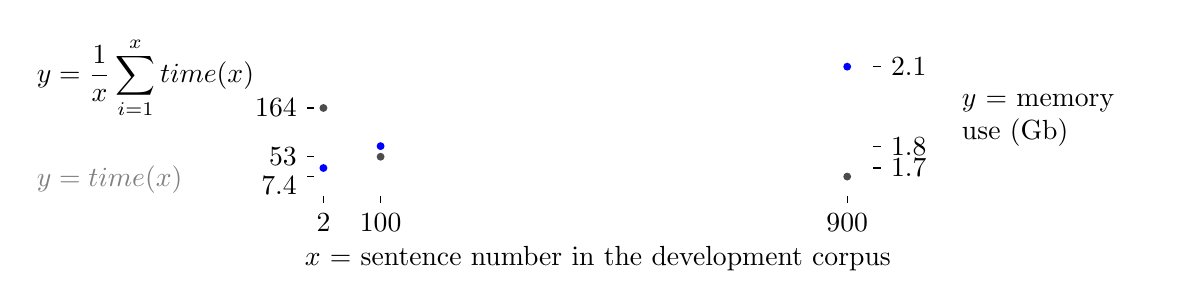
\begin{tikzpicture}
	%\draw[step=1,gray,very thin] (0,0) grid (10,3);
	%\draw[<->] (0,1.5) -- (0,0) -- (10,0);
	\node [anchor=east,text width=3.0cm] at (-0.5,1.3) {$\displaystyle y = \frac{1}{x}\sum_{i=1}^x time(x)$};
	\node [anchor=east,text width=2.5cm] at (-1,0) {\textcolor{gray}{$y = time(x)$}};
	\node [anchor=west,text width=2.5cm]  at (8,0.75) {$y$ = memory use (Gb)};
	\node at (3.5,-1.0) {$x$ = sentence number in the development corpus};
	\draw (0.0148148,-0.2) -- +(0.0,-0.1) node [anchor=north] {2};
	\draw (0.740741,-0.2) -- +(0.0,-0.1) node [anchor=north] {100};
	\draw (6.66667,-0.2) -- +(0.0,-0.1) node [anchor=north] {900};
	\draw[gray,thick] plot file {chap-algorithms/data-cache-by-sent};
	\draw[black,thick] plot file {chap-algorithms/data-cache-avg};
	\draw[blue,thick] plot file {chap-algorithms/data-cache-mem};
	
	\fill[blue] (0.0148148, 0.150011) circle (0.05);
	\fill[blue] (0.740741, 0.427965) circle (0.05);
	\fill[blue] (6.66667, 1.43709) circle (0.05);
	\draw (7.0,0.150011) -- +(0.1,0.0) node [anchor=west] {1.7};
	\draw (7.0,0.427965) -- +(0.1,0.0) node [anchor=west] {1.8};
	\draw (7.0,1.43709) -- +(0.1,0.0) node [anchor=west] {2.1};

	\fill[black!70] (0.0148148, 0.912278) circle (0.05);
	\fill[black!70] (0.740741, 0.293146) circle (0.05);
	\fill[black!70] (6.66667, 0.0412488) circle (0.05);
	\draw (-0.1,0.912278) -- +(-0.1,0.0) node[anchor=east] {164};
	\draw (-0.1,0.293146) -- +(-0.1,0.0) node[anchor=east] {53};
	\draw (-0.1,0.0412488) -- +(-0.1,0.0) node[anchor=east,text height=13pt] {7.4};
\end{tikzpicture}
